\bta{描绘电阻的伏安曲线}

\begin{enumerate}[leftmargin=0em]
\renewcommand{\labelenumi}{\arabic{enumi}.}
% A(\Alph) a(\alph) I(\Roman) i(\roman) 1(\arabic)
%设定全局标号series=example	%引用全局变量resume=example
%[topsep=-0.3em,parsep=-0.3em,itemsep=-0.3em,partopsep=-0.3em]
%可使用leftmargin调整列表环境左边的空白长度 [leftmargin=0em]
\item
小明想测额定电压为$ 2.5V $的小灯泡在不同电压下的电功率的电路。
\begin{figure}[h!]
\centering
\includesvg[width=0.23\linewidth]{picture/svg/664}
\end{figure}

\begin{enumerate}
\renewcommand{\labelenumi}{\arabic{enumi}.}
% A(\Alph) a(\alph) I(\Roman) i(\roman) 1(\arabic)
%设定全局标号series=example	%引用全局变量resume=example
%[topsep=-0.3em,parsep=-0.3em,itemsep=-0.3em,partopsep=-0.3em]
%可使用leftmargin调整列表环境左边的空白长度 [leftmargin=0em]
\item
($ 1 $)在实验过程中,调节滑片$ P $,电压表和电流表均有示数但总是调不到零,其原因是 \tk{$ 1 $点至$ 4 $点 } 
的导线没有连接好(图中用数字标记的小圆点表示接线点,空格中请填写图中的数字,如“$ 7 $点至$ 8 $点”);
\item 
正确连好电路,闭合开关,调节滑片$ P $,当电压表的示数达到额定电压时,电流表的指针如图所示,则电流为 \tk{$ 0,30 $} 
$ A $,此时小灯泡的功率为 \tk{$ 0.75 $} 
$ W $.
\begin{figure}[h!]
\centering
\includesvg[width=0.23\linewidth]{picture/svg/665}
\end{figure}

\item 
做完实验后小明发现在实验报告上漏写了电压为$ 1.00\ V $时通过小灯泡的电流,但在草稿纸上记录了下列数据,你认为最有可能的是 \xzanswer{C} 

\threechoices
{$ 0.08\ A $}
{$ 0.12\ A $}
{$ 0.20\ A $}




\end{enumerate}



\newpage
\item 
\exwhere{$ 2012 $年理综安徽卷}
图为“测绘小灯伏安特性曲线”实验的实物电路图,已知小灯泡额定电压为$ 2.5V $。
\begin{figure}[h!]
\centering
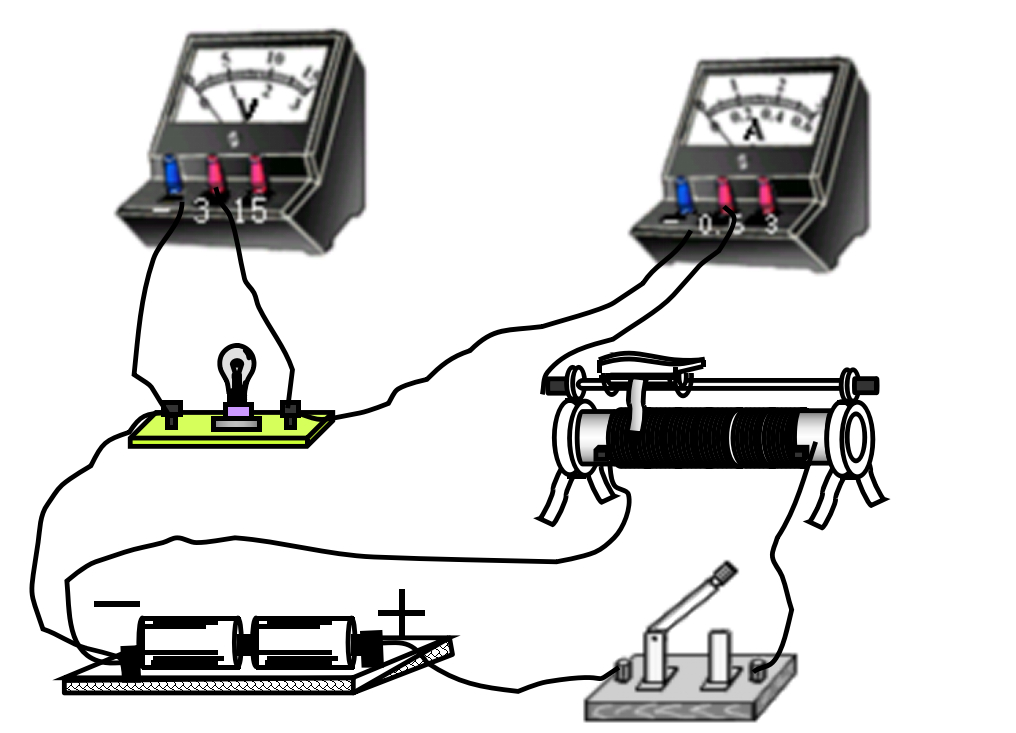
\includegraphics[width=0.5\linewidth]{picture/screenshot012}
\end{figure}

\begin{enumerate}
\renewcommand{\labelenumi}{\arabic{enumi}.}
% A(\Alph) a(\alph) I(\Roman) i(\roman) 1(\arabic)
%设定全局标号series=example	%引用全局变量resume=example
%[topsep=-0.3em,parsep=-0.3em,itemsep=-0.3em,partopsep=-0.3em]
%可使用leftmargin调整列表环境左边的空白长度 [leftmargin=0em]
\item
完成下列实验步骤:

①闭合开关前,调节滑动变阻器的滑片, \tk{它靠近变阻器左端的接线柱} 
; 

②闭合开关后,逐渐移动变阻器的滑片, \tk{增加小灯泡两端的电压,记录电流表和电压表的多组读数,直至电压达到额定电压} 
;

③断开开关,$ \cdots \cdots $ 。根据实验数据在方格纸上作出小灯泡灯丝的伏安特性曲线。
\item 
在虚线框中画出与实物电路相应的电路图。
\begin{figure}[h!]
\centering
\includesvg[width=0.23\linewidth]{picture/svg/668}
\end{figure}



\end{enumerate}


\banswer{
($ 2 $)电路图如图所示:
\includesvg[width=0.23\linewidth]{picture/svg/667}

}



\newpage
\item
\exwhere{$ 2013 $年天津卷}
要测绘一个标有“$ 3V 0.6W $”小灯泡的伏安特性曲线,灯泡两端的电压需要由零逐渐增加到$ 3V $,并便于操作。已选用的器材有:

电池组(电动势为$ 4.5V $,内阻约$ 1 \ \Omega ) $;

电流表(量程为$ 0 \sim 250 \ mA $.内阻约$ 5 \ \Omega ) $;

电压表(量程为$ 0 \sim 3V $.内限约$ 3 \ k\Omega ) $;

电键一个、导线若干。

①实验中所用的滑动变阻器应选下列中的 \tk{B} 

(填字母代号)。

A.滑动变阻器(最大阻值$ 20 \ \Omega $, 额定电流$ 1A $)

B.滑动变阻器(最大阻值$ 1750 \ \Omega $,额定电流$ 0.3A $)

②实验的电路图应选用下列的图 \tk{B} 

(填字母代号)。
\begin{figure}[h!]
\centering
\includesvg[width=0.83\linewidth]{picture/svg/669}
\end{figure}

③实脸得到小灯泡的伏安特性曲线如图所示。如果将这个小灯泡接到电动势为$ 1.5\ V $,内阻为$ 5 \ \Omega $的电源两端,小灯泡消耗的功率是 \tk{$ 0.1 $} 
$ W $。
\begin{figure}[h!]
\centering
\includesvg[width=0.43\linewidth]{picture/svg/670}
\end{figure}


\newpage
\item 
\exwhere{$ 2013 $年福建卷}
硅光电池在无光照时不产生电能,可视为一电子元件。某实验小组设计如图甲电路,给硅光电池加反向电压(硅光电池负极接高电势点,正极接低电势点),探究其在无光照时的反向伏安特性。图中电压表的$ V_{1} $量程选用$ 3V $,内阻为$ 6.0 \ k\Omega $;电压表$ V_{2} $量程选用$ 15V $,内阻约为$ 30 \ k\Omega $;$ R_{0} $为保护电阻;直流电源电动势$ E $约为$ 12V $,内阻不计。
\begin{figure}[h!]
\centering
\includesvg[width=0.83\linewidth]{picture/svg/671}
\end{figure}

\begin{enumerate}
\renewcommand{\labelenumi}{\arabic{enumi}.}
% A(\Alph) a(\alph) I(\Roman) i(\roman) 1(\arabic)
%设定全局标号series=example	%引用全局变量resume=example
%[topsep=-0.3em,parsep=-0.3em,itemsep=-0.3em,partopsep=-0.3em]
%可使用leftmargin调整列表环境左边的空白长度 [leftmargin=0em]
\item[①]
根据图甲,用笔画线代替导线,将图乙连接成完整电路。

\item [②]
用遮光罩罩住硅光电池,闭合开关$ S $,调节变阻器$ R $,读出电压表$ V_{1} $、$ V_{2} $的示教$ U_{1} $、$ U_{2} $。

\begin{enumerate}
\renewcommand{\labelenumi}{\arabic{enumi}.}
% A(\Alph) a(\alph) I(\Roman) i(\roman) 1(\arabic)
%设定全局标号series=example	%引用全局变量resume=example
%[topsep=-0.3em,parsep=-0.3em,itemsep=-0.3em,partopsep=-0.3em]
%可使用leftmargin调整列表环境左边的空白长度 [leftmargin=0em]
\item
某次测量时,电压表$ V_{1} $示数如图丙,则$ U_{1} = $ \tk{1.40} 
 $ V $,可算出通过硅光电他的反向电流大小为 \tk{0.23} 
 $ m_{A} $(保留两位小数)。
\item 
该小组测出大量数据,筛选出下表所示的$ 9 $组$ U_{1} $、$ U_{2} $数据,算出相应的硅光电池两端反向电压$ U_X $ 和通过反向电流$ I_X $(表中“$ - $”表示反向),并在坐标纸上建立$ I_x-U_x $坐标系,标出了与表中前$ 5 $组$ U_x $、$ I_x $数据对应的$ 5 $个坐标点。请你标出余下的$ 4 $个坐标点,并绘出$ I_x-U_x $图线。
\begin{table}[h!]
\centering 
\begin{tabular}{|c|c|c|c|c|c|c|c|c|c|}
\hline 
& 1 & 2 & 3 & 4 & 5 & 6 & 7 & 8 & 9
 \\
\hline
$ U_1/V $ & 0.00 & 0.00 & 0.06 & 0.12 & 0.24 & 0.42 & 0.72 & 1.14 & 1.74
 \\
\hline
$ U_2/V $ & 0.0 & 1.0 & 2.1 & 3.1 & 4.2 & 5.4 & 6.7 & 8.1 & 9.7
 \\
\hline
$ U_x/V $ & 0.0 & -1.0 & -2.0 & -3.0 & -4.0 & -5.0 & -6.0 & -7.0 & -8.0
 \\
\hline
$ I_x/mA $ & -0.00 & -0.00 & -0.01 & -0.02 & -0.04 & -0.07 & -0.12 & -0.19 & -0.29\\ 
\hline 
\end{tabular}\\
\includesvg[width=0.63\linewidth]{picture/svg/673} 
\end{table} 

\item 
由$ I_x-U_x $图线可知,硅光电池 无光照下加反向电压时, $ I_x $与$ U_x $成 \tk{非线性} 
( 填“线性”或“非线性” )关系。



\end{enumerate}




\end{enumerate}

\banswer{
①电路连接如答图$ 1 $所示 :
\includesvg[width=0.23\linewidth]{picture/svg/672}

$ I_x-U_x $图线 如答图$ 2 $所示 :
 \includesvg[width=0.23\linewidth]{picture/svg/674} 
}


\newpage
\item 
\exwhere{$ 2011 $年理综福建卷}
某同学在探究规格为“$ 6\ V $,$ 3\ W $”的小电珠伏安特性曲线实验中:
\begin{figure}[h!]
\centering
\includesvg[width=0.23\linewidth]{picture/svg/675} \qquad \qquad 
 \includesvg[width=0.23\linewidth]{picture/svg/676} 
\end{figure}

①在小电珠接入电路前,使用多用电表直接测量小电珠的电阻,则应将选择开关旋至 \xzanswer{D} 
档进行测量。(填选项前的字母)
\fourchoices
{直流电压$ 10V $ }
{直流电流$ 5 \ mA $}
{欧姆$ \times $ $ 100 $ }
{欧姆$ \times $ $ 1 $}

②该同学采用图甲所示的电路进行测量。图中$ R $为滑动变阻器(阻值范围$ 0 \sim 20 \ \Omega $,额定电流$ 1.0A $),$ L $为待测小电珠, \voltmetermytikz 为电压表(量程$ 6V $,内阻$ 20 \ k\Omega $), \ammetermytikz 为电流表(量程$ 0.6A $,内阻$ 1 \ \Omega $),$ E $为电源(电动势$ 8V $,内阻不计),$ S $为开关。

$ \lmd{1} $.在实验过程中,开关$ S $闭合前,滑动变阻器的滑片$ P $应置于最 \tk{左} 
端;(填“左”或“右”)

$ \lmd{2} $.在实验过程中,已知各元器件均无故障,但闭合开关$ S $后,无论如何调节滑片$ P $,电压表和电流表的示数总是调不到零,其原因是 \tk{1} 
点至 \tk{5} 
点的导线没有连接好;(图甲中的黑色小圆点表示接线点,并用数字标记,空格中请填写图甲中的数字,如“$ 2 $点至$ 3 $点”的导线)

$ \lmd{3} $.该同学描绘出小电珠的伏安特性曲线示意图如图乙所示,则小电珠的电阻值随工作电压的增大而 \tk{增大} 
。(填“不变”、“增大”或“减小”)


\item 
\exwhere{$ 2015 $年理综浙江卷}
图$ 1 $是小红同学在做“描绘小灯泡的伏安特性曲线”实验的实物连接图。
\begin{figure}[h!]
\centering
\includesvg[width=0.83\linewidth]{picture/svg/677}
\end{figure}

\begin{enumerate}
\renewcommand{\labelenumi}{\arabic{enumi}.}
% A(\Alph) a(\alph) I(\Roman) i(\roman) 1(\arabic)
%设定全局标号series=example	%引用全局变量resume=example
%[topsep=-0.3em,parsep=-0.3em,itemsep=-0.3em,partopsep=-0.3em]
%可使用leftmargin调整列表环境左边的空白长度 [leftmargin=0em]
\item
根据图$ 1 $画出实验电路图
\item 
调节滑动变阻器得到了两组电流表与电压表的示数如图$ 2 $中的①、②、③、④所示,电流表量程为$ 0.6\ A $,电压表量程为$ 3\ V $。所示读数为:

① \tk{0.10 A} 
② \tk{0.24 A} 
③ \tk{2.00 V} 
④ \tk{0.27 V} 
。两组数据得到的电阻分别为 \tk{($ 8.3\pm 0.1 $)$ \Omega $} 
和 \tk{($ 2.7\pm 0.1 $)$ \Omega $} 
。





\end{enumerate}

\banswer{
答案如图$ 1 $所示:
 \includesvg[width=0.23\linewidth]{picture/svg/679} 
}


\newpage
\item 
\exwhere{$ 2016 $年天津卷}
某同学想要描绘标有“$ 3.8\ V $,$ 0.3\ A $”字样小灯泡$ L $的伏安特性曲线,要求测量数据尽量精确,绘制曲线完整,可供该同学选用的器材除了开关,导线外,还有:

电压表$ V_{1} $(量程$ 0 \sim 3V $,内阻等于$ 3 \ k\Omega $)

电压表$ V_{2} $(量程$ 0 \sim 15V $,内阻等于$ 15 \ k\Omega $)

电流表$ A_{1} $(量程$ 0 \sim 200 \ mA $,内阻等于$ 10 \ \Omega $)

电流表$ A_{2} $(量程$ 0 \sim 3A $,内阻等于$ 0.1 \ \Omega $)

滑动变阻器$ R_{1} $($ 0 \sim 10 \ \Omega $,额定电流$ 2A $)

滑动变阻器$ R_{2} $($ 0 \sim 1 \ k\Omega $,额定电流$ 0.5A $)

定值电阻$ R_{3} $(阻值等于$ 1 \ \Omega $)

定值电阻$ R_{4} $(阻值等于$ 10 \ \Omega $)

定值电阻$ R_{5} $(阻值等于$ 1 \ k\Omega $)

电源$ E $,($ E=6V $,内阻不计)

①请画出实验电路图,并将各元件字母代码标在该元件的符号旁.

②该同学描绘出的$ I-U $图像应是下图中的 \tk{B} 
\begin{figure}[h!]
\centering
\includesvg[width=0.63\linewidth]{picture/svg/680}
\end{figure}

\banswer{
①电路如图:
 \includesvg[width=0.23\linewidth]{picture/svg/681} 
}

\item 
\exwhere{$ 2011 $年理综重庆卷}
在测量电珠伏安特性实验中,同学们连接的电路中有四个错误电路,如图所示。电源内阻不计,导线连接良好。若将滑动变阻器的触头置于左端,闭合$ S $,在向右端滑动触头过程中,会分别出现如下四种现象:
\begin{figure}[h!]
\centering
\includesvg[width=0.83\linewidth]{picture/svg/683}
\end{figure}

$ a $.电珠$ L $不亮;电流表示数几乎为零;

$ b $.电珠$ L $亮度增加;电流表示数增大;

$ c $.电珠$ L $开始不亮;后来忽然发光;电流表从示数不为零到线圈烧断;

$ d $.电珠$ L $不亮;电流表从示数增大到线圈烧断。

与上述$ abcd $四种现象对应的电路序号为 \xzanswer{A} 

\fourchoices
{③①②④ }
{③④②①}
{③①④② }
{②①④③}


\newpage
\item 
\exwhere{$ 2011 $年理综广东卷}
在“描绘小电珠的伏安特性曲线”实验中,所用器材有:小电珠($ 2.5V $,$ 0.6W $),滑动变阻器,多用电表,电流表,学生电源,开关,导线若干。
\begin{figure}[h!]
\centering
\includesvg[width=0.83\linewidth]{picture/svg/682}\\
\vspace{2em}
 \begin{tabular}{|c|c|c|c|c|c|c|}
\hline 
数据点 & a & b & c & d & e & f
 \\
\hline
U/V & 0.00 & 0.50 & 1.00 & 1.50. & 2.00 & 2.50\\ 
\hline 
\end{tabular}
\end{figure}




①粗测小电珠的电阻,应选择多用电表倍率的电阻档 \tk{ $ \times 1 $} 
(请填写“$ \times 1 $”、“$ \times 10 $”或“$ \times 100 $”);调零后,将表笔分别与小电珠的两极连接,示数如图$ (c) $,结果为$ \Omega $。 

②实验中使用多用电表测量电压,请根据实验原理图$ (d) $完成实物图$ (e) $中的连线。

③开关闭合前,应将滑动变阻器的滑片$ P $置于 \tk{$ a $} 
端。为使小电珠亮度增加,$ P $应由中点向 \tk{$ b $} 
端滑动。

④下表为电压等间隔变化测得的数据,为了获得更准确的实验图象,必须在相邻数据点 \tk{ab} 
间多测几组数据(请填写“$ ab $”、“$ bc $”、“$ cd $”、“$ de $”或“$ ef $”)

\banswer{
②电流表的电阻也就几欧,与电压表几千欧相比,小电珠算小电阻,所以电压表必须外接,伏安特性曲线要求电压从0开始逐渐变大,所以滑动变阻器必须与电压采用分压接法。
}




\item 
\exwhere{$ 2012 $年理综重庆卷}
某中学生课外科技活动小组利用铜片、锌片和家乡盛产的柑橘制作了果汁电池,他们测量这种电池的电动势$ E $和内阻$ r $,并探究电极间距对$ E $和$ r $的影响。实验器材如图$ 3 $所示。
\begin{figure}[h!]
\centering
\includesvg[width=0.43\linewidth]{picture/svg/684}
\end{figure}


①测量$ E $和$ r $的实验方案为:调节滑动变阻器,改变电源两端的电压$ U $和流过电源的电流 \lmd{1} ,依据公式 \tk{$U = E - I r$} 
,利用测量数据作出$ U-I $ 图象,得出$ E $和$ r $。

②将电压表视为理想表,要求避免电流表分压作用对测量结果的影响,请在题图$ 3 $中用笔画线代替导线连接电路。 

③实验中依次减小铜片与锌片的间距,分别得到相应果汁电池的$ U-I $ 图象如图$ 4 $(见下图)中($ a $)、($ b $)、($ c $)、($ d $)所示,由此可知:
\begin{figure}[h!]
\centering
\includesvg[width=0.63\linewidth]{picture/svg/685}
\end{figure}

在该实验中,随电极间距的减小,电源电动势 \tk{不变} 
(填“增大”、“减小”或“不变”),电源内阻 \tk{增大} 
(填“增大”、“减小”或“不变”)。

曲线($ c $)对应的电源电动势$ E= $ \tk{0.975} 
$ V $,内阻$ r= $ \tk{480} 
$ \Omega $,当外电路总电阻为$ 2500 \ \Omega $时,该电源的输出功率$ P= $ \tk{267} 
$ mW $。(均保留三位有效数字)

\banswer{
②见题答图
 \includesvg[width=0.23\linewidth]{picture/svg/686} 
}


\newpage
\item 
\exwhere{$ 2015 $年理综福建卷}
某学习小组探究一小电珠在不同电压下的电功率大小,实验器材如图甲所示,现已完成部分导线的连接。
\begin{figure}[h!]
\centering
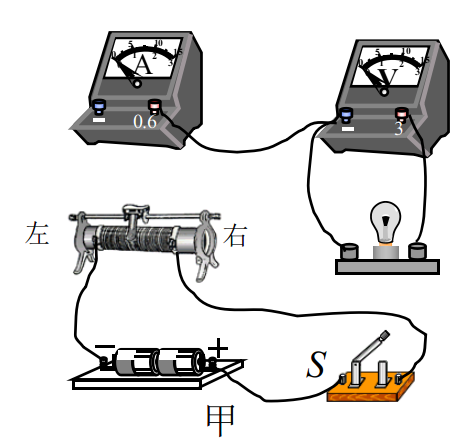
\includegraphics[width=0.37\linewidth]{picture/screenshot013} \qquad 
\includesvg[width=0.47\linewidth]{picture/svg/687} 
\end{figure}



①实验要求滑动变阻器的滑片从左到右移动过程中,电流表的示数从零开始逐渐增大,请按此要求用笔画线代替导线在图甲实物接线图中完成余下导线的连接;

②某次测量,电流表指针偏转如图乙所示,则电流表的示数为 \tk{0.44} 
$ A $;

③该小组描绘出的伏安特性曲线如图丙所示,根据图线判断,将 \tk{4} 
只相同的小电珠并联后,直接与电动势为$ 3V $、内阻为$ 1 \ \Omega $的电源组成闭合回路,可使小电珠的总功率最大,其总功率的值约为 \tk{$ 2.22 \sim 2.28 $} 
$ W $(保留两位小数)。


\banswer{
①连线如图:
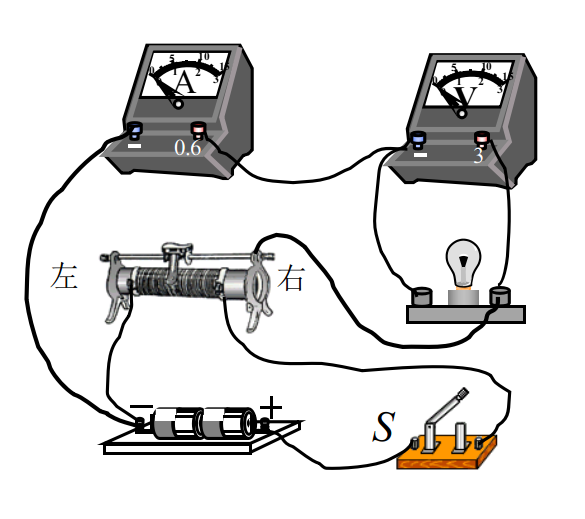
\includegraphics[width=0.7\linewidth]{picture/screenshot014} 
}




\item 
\exwhere{$ 2017 $年新课标 \lmd{1} 卷}
某同学研究小灯泡的伏安特性,所使用的器材有:小灯泡$ L $(额定电压$ 3.8 $ $ V $,额定电流$ 0.32 $ $ A $);电压表 \voltmetermytikz (量程$ 3 $ $ V $,内阻$ 3 $ $ k \Omega $);电流表 \ammetermytikz (量程$ 0.5 $ $ A $,内阻$ 0.5 $ $ \Omega $);固定电阻$ R_{0} $(阻值$ 1000 $ $ \Omega $);滑动变阻器$ R $(阻值$ 0 \sim 9.0 $ $ \Omega $);电源$ E $(电动势$ 5 $ $ V $,内阻不计);开关$ S $;导线若干。


\begin{enumerate}
\renewcommand{\labelenumi}{\arabic{enumi}.}
% A(\Alph) a(\alph) I(\Roman) i(\roman) 1(\arabic)
%设定全局标号series=example	%引用全局变量resume=example
%[topsep=-0.3em,parsep=-0.3em,itemsep=-0.3em,partopsep=-0.3em]
%可使用leftmargin调整列表环境左边的空白长度 [leftmargin=0em]
\item
实验要求能够实现在$ 0 \sim 3.8 $ $ V $的范围内对小灯泡的电压进行测量,画出实验电路原理图。

\item 
实验测得该小灯泡伏安特性曲线如图($ a $)所示。
由实验曲线可知,随着电流的增加小灯泡的电阻 \tk{增大} 
(填“增大”“不变”或“减小”),灯丝的电阻率 \tk{增大} 
(填“增大”“不变”或“减小”)。
\begin{figure}[h!]
\centering
\includesvg[width=0.33\linewidth]{picture/svg/690}
\end{figure}

\item 
用另一电源$ E_{0} $(电动势$ 4 $ $ V $,内阻$ 1.00 $ $ \Omega $)和题给器材连接成图($ b $)所示的电路,调节滑动变阻器$ R $的阻值,可以改变小灯泡的实际功率。闭合开关$ S $,在$ R $的变化范围内,小灯泡的最小功率为 \tk{0.39} 
$ W $,最大功率为 \tk{1.17} 
$ W $。(结果均保留$ 2 $位小数)




\end{enumerate}

\banswer{
($ 1 $)如答图$ 1 $示:
\includesvg[width=0.23\linewidth]{picture/svg/691} 
}


\newpage

\item
\exwhere{$ 2015 $年广东卷}
某实验小组研究两个未知元件$ X $和$ Y $的伏安特性,使用的器材包括电压表(内阻约为$ 3 \ k\Omega $)、电流表(内阻约为$ 1 \ \Omega $)、定值电阻等。

①使用多用电表粗测元件$ X $的电阻。选择“$ \times 1 $”欧姆档测量,示数如图($ a $)所示,读数为 \tk{10} 
$ \Omega $。据此应选择图中的 \tk{b} 
(填“$ b $”或“$ c $”)电路进行实验。
\begin{figure}[h!]
\centering
\includesvg[width=0.83\linewidth]{picture/svg/688}
\end{figure}

②连接所选电路,闭合$ S $;滑动变阻器的滑片$ P $从左向右滑动,电流表的示数逐渐 \tk{增大} 
(填“增大”或“减小”);依次记录电流及相应的电压;将元件$ X $换成元件$ Y $,重复实验。

③下图($ a $)是根据实验数据作出的$ U-I $图线,由图可判断元件 \tk{Y} 
(填“$ X $”或“$ Y $”)是非线性元件。
\begin{figure}[h!]
\centering
\includesvg[width=0.43\linewidth]{picture/svg/689}
\end{figure}

④该小组还借助$ X $和$ Y $中的线性元件和阻值$ R=21 \ \Omega $的定值电阻,测量待测电池组的电动势$ E $和电阻$ r $,如图($ b $)所示。闭合$ S_{1} $和$ S_{2} $,电压表读数为$ 3.00V $;断开$ S_{2} $,读数为$ 1.00V $,利用图($ a $)可算得$ E= $ \tk{3.2} 
$ V $,$ r= $ \tk{0.50} 
$ \Omega $(结果均保留两位有效数字,视电压表为理想电压表)。



\newpage 







\end{enumerate}

